
\chapter{Aplicação do Procedimento}

Neste capítulo o procedimento será ilustrado em um modelo de regressão de preços de imóveis. Todos os dados e código de implementação estão disponíveis sob a licensa MIT no repositório https://github.com/pedrocava/monografiaRandomForest. Os dados foram adquiridas via \textit{webscrapping} de um site nacional de aluguel de imóveis (https://www.quintoandar.com.br) para quatro capitais brasileiras no dia 20 de Março de 2020, realizado pelo autor. Iremos realizar análise exploratória para entender melhor os dados de alugueis, estimar uma série de modelos com variadas configurações de hiperparâmetros e computar algumas métricas de sucesso para explorar como eles afetam performance do modelo. Essas métricas de sucesso serão computadas com dados omitidos no processo de treinamento, num processo chamado Validação Cruzada, e então aplicaremos o procedimento descrito no capítulo anterior. 


Antes, no entanto, veremos o procedimento ser aplicado em um contexto laboratorial. Simularemos dados aleatórios a partir de um modelo linear e recuperaremos o parâmetro estimado com florestas aleatórias e uma aplicação do procedimento. 


\section{Verificação Laboratorial}

Para uma primeira verificação da sanidade da técnica apresentada, o seguinte procedimento será feito. Primeiro dados aleatórios serão gerados a partir de uma normal. Esse será nosso regressor. Depois serão simulados outros dados de uma normal, que serão os erros. Depois, um cálculo determinístico irá gerar a nossa resposta simulada com um parâmetro conhecido. 

Será treinada uma floresta aleatória nessa amostra falsificada e suas previsões serão computadas para variados valores do regressor imaginário. Iremos, então, estimar uma regressão linear do regressor simulado original nas predições da floresta aleatória. Caso a floresta de fato tenha conseguido recuperar o parâmetro, o $\beta$ que escolhemos para o cálculo determinístico da resposta deverá ser o mesmo que encontraremos na segunda regressão. 

As Figuras 6, 7 e 8 descrevem, respectivamente: a distribuição conjunta dos dados simulados, o resultado da aplicação do procedimento de computação de efeitos marginais ao lado da curva de predição média e a distribuição conjunta dos valores preditos pelo modelo de floresta aleatória com os verdadeiros. Há uma relação aparentemente 1 para 1, o que é um sinal muito positivo já antes de verificar os resultados.


\begin{figure}[H]
    \centering
    \captionbox{Dados simulados.  }{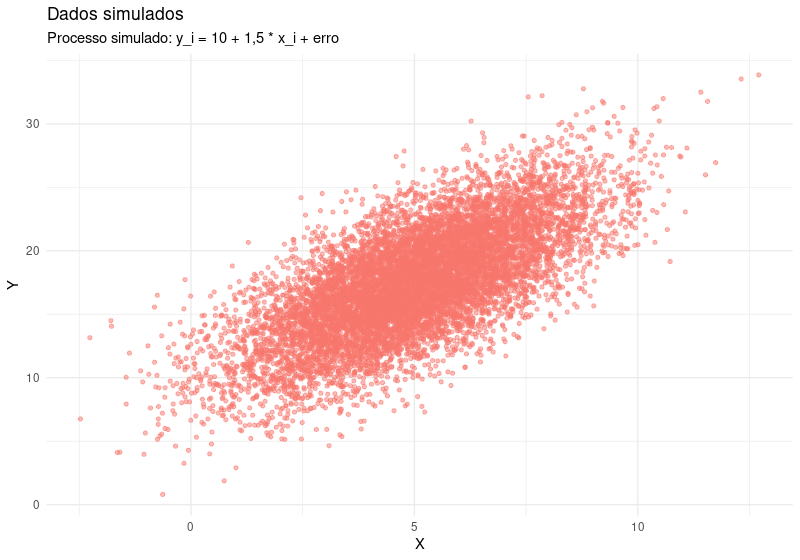
\includegraphics[scale = .75]{imagens/exemplo_freddy_fake_data.png}}
\fonte{Elaboração própria.}
\end{figure}



\begin{figure}[H]
    \centering
    
    \captionbox{Comportamento dos efeitos marginais, que lembra um ruído branco, e a curva de predições.  }{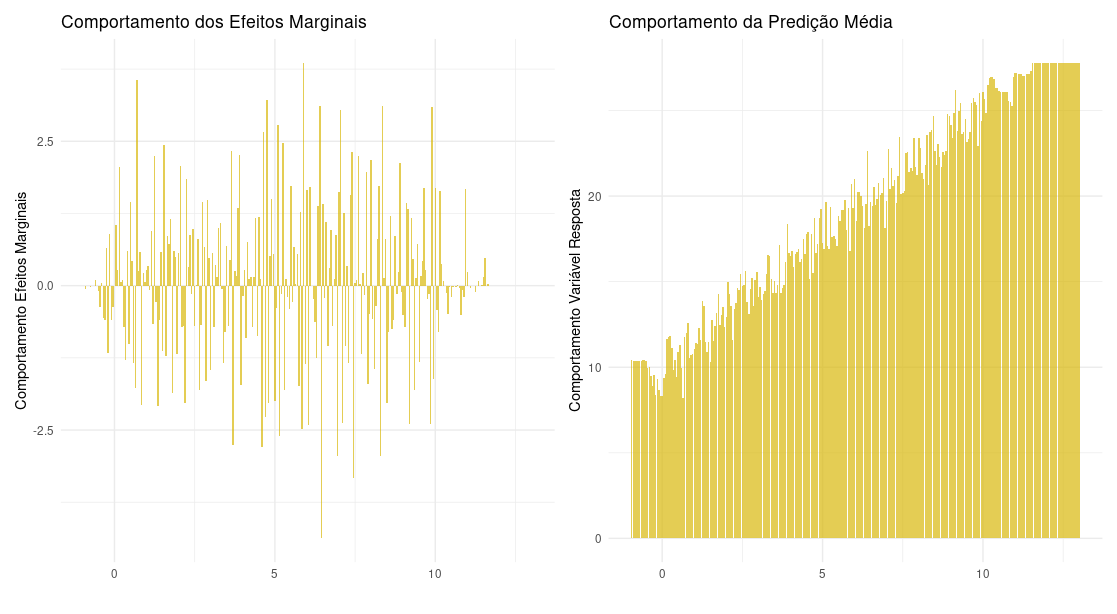
\includegraphics[scale = .50]{imagens/exemplo_freddy_efeitos_marginais.png}}
    \fonte{Elaboração própria.}
\end{figure}


\begin{figure}[H]
    \centering
    
    \captionbox{Comparação das predições com os valores verdadeiros.  }{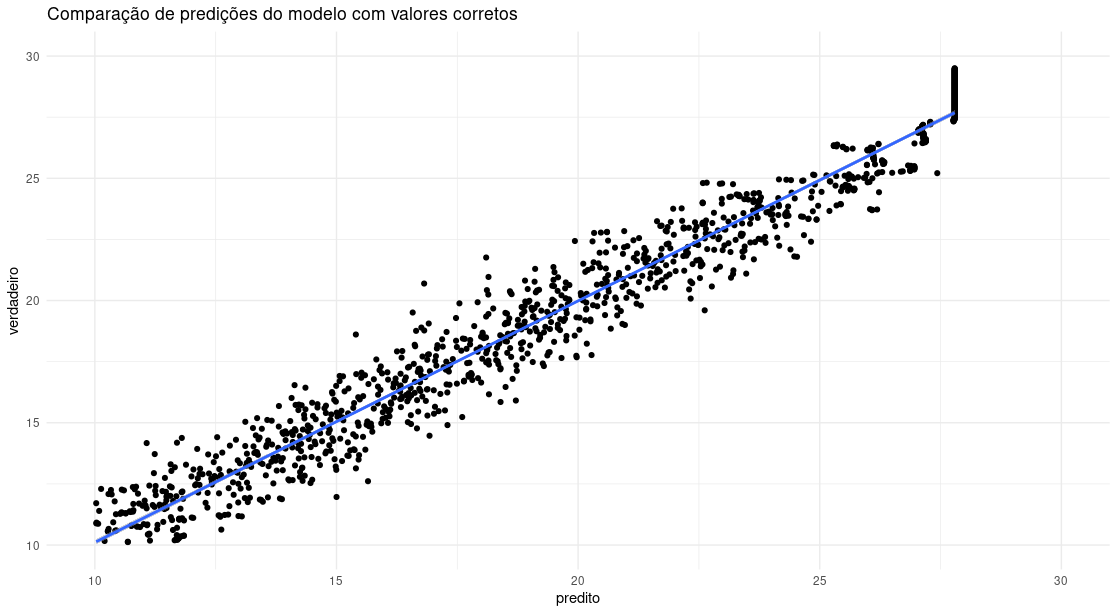
\includegraphics[scale = .55]{imagens/exemplo_freddy_predito_vs_verdade.png}}
\fonte{Elaboração própria.}
\end{figure}

Na Tabela \ref{tabela_verif} estão os resultados para a segunda regressão do experimento. Ao gerar a resposta simulada, escolhemos um $\beta$ de exatamente $1.5$. Nosso procedimento recuperou esse parâmetro com um erro de cerca de $2,5\%$.


% Table created by stargazer v.5.2.2 by Marek Hlavac, Harvard University. E-mail: hlavac at fas.harvard.edu
% Date and time: Sat, Feb 13, 2021 - 11:34:16 PM
\begin{table}[!htbp] \centering 
  \caption{} 
  \label{} 
\begin{tabular}{@{\extracolsep{5pt}}lc} 
\\[-1.8ex]\hline 
\hline \\[-1.8ex] 
 & \multicolumn{1}{c}{\textit{Dependent variable:}} \\ 
\cline{2-2} 
\\[-1.8ex] & predito \\ 
\hline \\[-1.8ex] 
 X & 1.465$^{***}$ \\ 
  & (0.007) \\ 
  & \\ 
 Constant & 10.243$^{***}$ \\ 
  & (0.050) \\ 
  & \\ 
\hline \\[-1.8ex] 
Observations & 1,401 \\ 
R$^{2}$ & 0.970 \\ 
Adjusted R$^{2}$ & 0.970 \\ 
Residual Std. Error & 1.046 (df = 1399) \\ 
F Statistic & 44,946.980$^{***}$ (df = 1; 1399) \\ 
\hline 
\hline \\[-1.8ex] 
\textit{Note:}  & \multicolumn{1}{r}{$^{*}$p$<$0.1; $^{**}$p$<$0.05; $^{***}$p$<$0.01} \\ 
\end{tabular} 
\end{table} 



\section{Exploração dos Dados de Imóveis}

Nesta seção algumas visualizações de dados úteis serão apresentadas, bem como uma descrição dos dados. Foram mensuradas as seguintes variáveis:

\begin{itemize}
    \item \textbf{Cidade:} a cidade onde está o apartamento.
    \item \textbf{Área:} a área em metros quadrados
    \item \textbf{Quartos:} o número de quartos
    \item \textbf{Banheiros:} o número de banheiros
    \item \textbf{Vagas:} o número de vagas
    \item \textbf{Andar:} em qual andar do prédio está o apartamento (0 para térreo ou casas)
    \item \textbf{Mobiliado:} variável categórica indicando se o apartamento é mobiliado
    \item \textbf{Aluguel:} valor do aluguel em reais por mês
\end{itemize}

Na Tabela \ref{tab:exploratoria} algumas estatísticas descritivas importantes por cidade e alguns gráficos descrevendo as variáveis chaves.

\begin{table}[H]
\caption{\label{tab:exploratoria} Estatísticas descritivas por cidade.}
\begin{tabular}{l|r|r|r|r}

\hline
Cidade & Área Média & Quartos $/$ apt & Aluguel Médio & Custo Médio por M^2\\
\hline
Belo Horizonte & 136.71 & 2.9 & 2765.90 & 22.81\\
\hline
Porto Alegre & 93.27 & 2.0 & 2069.88 & 25.29\\
\hline
Rio de Janeiro & 93.14 & 2.1 & 2774.70 & 34.18\\
\hline
São Paulo & 124.69 & 2.4 & 3600.26 & 37.62\\
\hline
\end{tabular}
    \fonte{Cálculos do autor com dados raspados do site https://quintoandar.com.br.}
\end{table}



\begin{figure}[H]
    \centering
    
    \captionbox{Distribuição dos aluguéis.  }{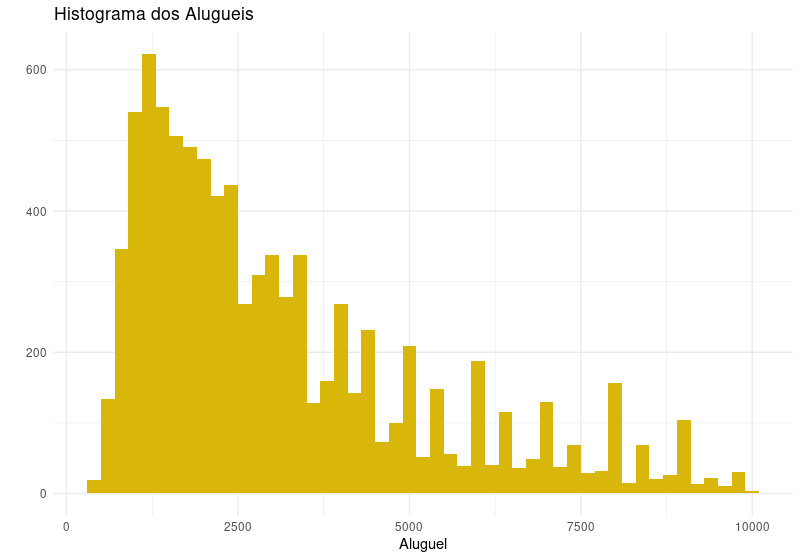
\includegraphics[scale = .65]{imagens/exploratoria_alugueis.png}}
    \fonte{Cálculos do autor com dados raspados do site https://quintoandar.com.br.}
\end{figure}

\begin{figure}[H]
    \centering
    
    \captionbox{Distribuição dos andares dos apartamentos.  }{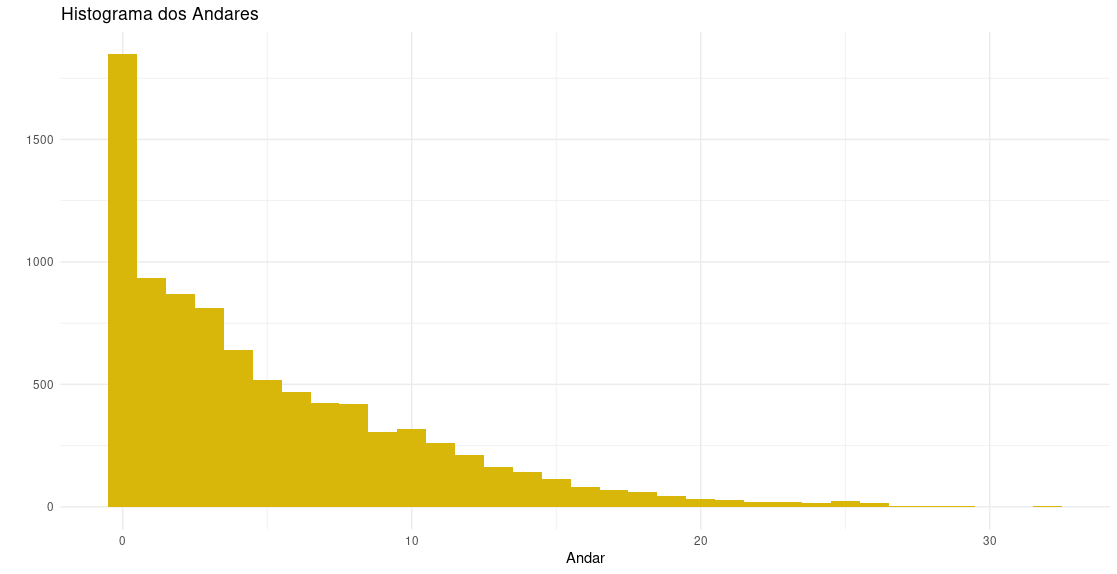
\includegraphics[scale = .55]{imagens/exploratoria_andares.png}}
        \fonte{Cálculos do autor com dados raspados do site https://quintoandar.com.br.}
\end{figure}

\begin{figure}[H]
    \centering
    
    \captionbox{Distribuição da metragem dos apartamentos.  }{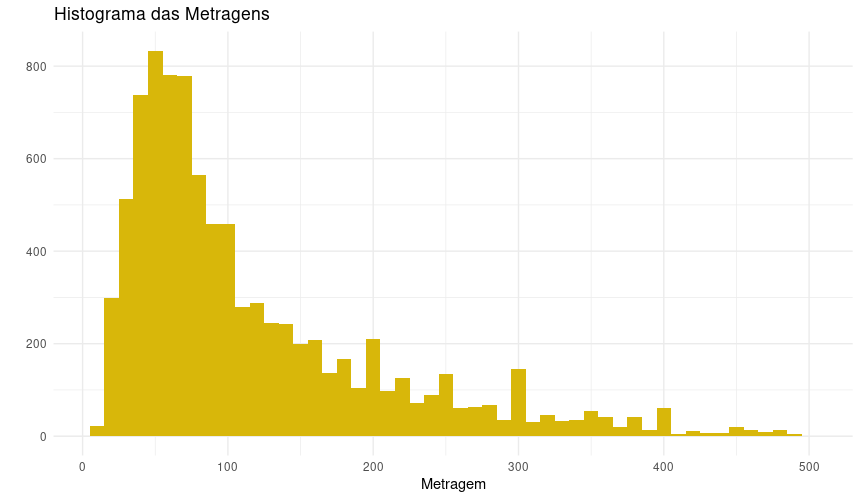
\includegraphics[scale = .65]{imagens/exploratoria_metragens.png}}
        \fonte{Cálculos do autor com dados raspados do site https://quintoandar.com.br.}
\end{figure}


\section{Otimização de hiperparâmetros}

Não existe uma única maneira de estimar uma floresta aleatória. De fato, como machine learning é um campo que cresceu muito às margens da academia, em laboratórios da indústria, as convenções são informais e há pouco escrito em pedra. Optei por usar a implementação em \citeonline{ranger}, que usa como gatilho de geração de folhas uma amostra abaixo da mínima chegar no nodo e aleatoriza quantas variáveis explicativas são usadas em cada árvore. Uma alternativa de alta confiabilidade seria \citeonline{randomForest}. Para a otimização de hiperparâmetros, validação cruzada e avaliação dos modelos foi usada a plataforma \texttt{tidymodels} \cite{tidymodels}, implementada em linguagem R \cite{R}.

Decidida a implementação que irá realizar as computações, é preciso fazer uma escolha sobre os hiperparâmetros do modelo, no caso três: amostra mínima para criação de folha, número de árvores e número de variáveis a serem aleatoriamente escolhidas para cada árvore. Do ponto de vista do expectador desinteressado o problema é apenas:

\begin{align}
    \mathbf{x}^* = \underset{\mathbf{x}}{\text{arg max}} \,\,\phi(\mathbf{x}) 
\end{align}

E como seria fácil se soubéssemos exatamente o que é $\phi(\cdot)$, mas não sabemos. Uma primeira abordagem é tatear o suporte da função em busca da melhor combinação. Um método para isso é \textit{random search}, gerar algumas combinações de hiperparâmetros aleatórias, estimar um modelo em cada e escolher o de melhor performance, que definiremos em detalhes brevemente. O dual dessa abordagem é \textit{grid search} em que ao invés de gerar combinações aleatórias se cobre o espaço de hiperparâmetros de vetores com distância regular, gerando uma grade. 

Essas são ditas abordagens \textbf{caixa-preta livre de modelo} pois não fazem suposições sobre a forma funcional da função a ser maximizada ajustando os hiperparâmetros. Varremos o que acreditamos ser o seu domínio à força bruta. Existem alternativas, \citeonline{shahriari2015taking} é um tratamento amplo da principal, otimização bayesiana. Otimização de Hiperparâmetros é um campo vasto. Um tratamento mais detalhado do estado da arte na área está disponível em \citeonline{feurer2019hyperparameter}.


\begin{figure}[H]
    \centering
    
    \captionbox{Duas buscas de 100 modelos cada.  }{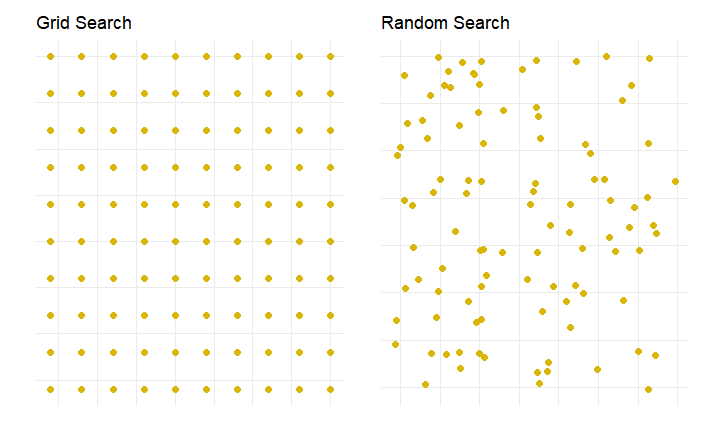
\includegraphics[scale = .75]{imagens/random_grid.png}}
        \fonte{Elaboração própria.}
\end{figure}

\section{Métricas de Qualidade}

Na seção anterior optamos por escolher hiperparâmetros de forma a maximizar alguma função que entendemos representar a qualidade de um modelo. Precisamos agora definir como mensura-la. Métricas de performance de modelo são sempre arbitrárias então a boa prática recomenda usar uma cesta delas. As opções para regressão são inúmeras. Serão avaliadas seis: 

\begin{itemize}
    \item \textbf{Razão Performance-Interquatil (RPIQ)} \newline
    Definida como o desvio-padrão das previsões dividido pela amplitude interquartil observada da resposta. Mede a capacidade do modelo de gerar previsões parcimoniosas. Quanto mais próximo de 1, melhor. Um tratamento mais detalhado está disponível em \citeonline{botchkarev2018performance}.
    
    \item \textbf{Coeficiente de Concordância de Correlação (CCC)} \newline
    Introduzido por \citeonline{lawrence1989concordance}, mede acurácia. Calculada a partir da diferença entre a identidade e a reta de regressão dos valores preditos nos observados. Quanto mais próximo de 1, melhor.
    
    \item \textbf{Erro Médio Absoluto (MAE)} \newline
    A média das diferenças entre previsões e valores observados. Diretamente interpretável na unidade original da resposta. Indica acurácia. Menor é melhor, mas deve-se atentar à parcimônia.
    
    \item \textbf{Erro Médio Percentual (MPE)} \newline
    A média das diferenças entre previsões e valores observados ponderada pela média da resposta. Lida em unidades relativas. Indica acurácia. Menor é melhor, mas deve-se atentar à parcimônia.
    
    \item \textbf{Coeficiente de Determinação (R2)} \newline
    Calcula-se a soma dos quadrados dos desvios das previsões à média da resposta. Dividi-se esse valor pela soma dos quadrados dos desvios as observações originais à média da resposta. O resultado está entre $0$ e $1$ e pode ser interpretado como a fração da variância que o modelo consegue explicar. Maior é melhor, mas deve-se atentar à parcimônia, pois cresce monotonamente no número de variáveis explicativas.
    
    Uma variante dessa métrica, especialmente apropriada para comparar modelos com os mesmos hiperparâmetros (ou que não dependam deles, como regressão linear) e variáveis explicativas diferentes é o R2 ajustado. Seu cálculo é muito similar, mas introduz um mecanismo de punição à adição de variáveis, refletindo os benefícios da parcimônia na métrica.
    
    
    \item \textbf{Raiz do Erro Quadrático Médio (RMSE)} \newline
    O Erro Quadrático Médio é a média dos quadrados dos desvios das previsões em relação aos valores observados. A raiz dá a métrica. Mede principalmente acurácia, embora seja muito sensível a outliers. Menor é melhor.
    
\end{itemize}

Em um contexto de classificação precisamos de outras métricas. A título de exemplo, algumas das mais amplamente utilizadas são:

\begin{itemize}
    \item \textbf{Sensitividade/ Recall} \newline
    Em classificação binária, a Sensitividade é a proporção dos casos positivos que são corretamente identificados.
    \item \textbf{Especificidade} \newline
    Em classificação binária, a Especificidade é a proporção dos casos negativos que são corretamente identificados.
    \item \textbf{Acurácia} \newline
    A fração de casos corretamente identificados. 
    \item \textbf{Precisão/ Valor Preditivo Positivo} \newline
    O número de observados positivos dividido pelo número de preditos positivos.
    \item \textbf{F1-Score} \newline
    Média harmônia da Precisão e da Sensitividade
\end{itemize}


\section{Validação Cruzada}

Para dar uma chance melhor a cada combinação podemos testa-la em amostras diferentes. Fazemos isso com validação $k$-cruzada. Dividimos a amostra em $k$ grupos aproximadamente iguais e para cada combinação de hiperparâmetros estimamos o modelo em $k-1$ combinações, excluindo um grupo de cada vez. Como medida de performance para cada combinação específica de hiperparâmetros usamos então a média das métricas de performance nas $k-1$ validações. 

A literatura da área sugere que o número de árvores não é um bom hiperparâmetro para se validar  \cite{claesen2015hyperparameter}. Os ganhos de performance são pequenos, o custo computacional, no entanto, variante. Note que o custo de estimar uma floresta cresce linearmente, um para um, com o número de árvores. Validar $k$ combinações cada uma com $a*b$ árvores é $a$ vezes mais caro que validar $k$ combinações com $b$ árvores. 

Esse tempo de computação é melhor empregado procurando com uma grade fina melhores combinações de amostra única e número de variáveis por árvore. Árvores com menos variáveis tem menos variância, o que ajuda a diminuir a variância da floresta, e menor poder preditivo. Árvores com menor amostra mínima têm mais folhas, criando respostas mais finas, mas têm mais variância também. 


\begin{figure}[H]
    \centering
    
    \captionbox{Resumo de métricas de performance variando quantas variáveis alimentar para cada árvore.  }{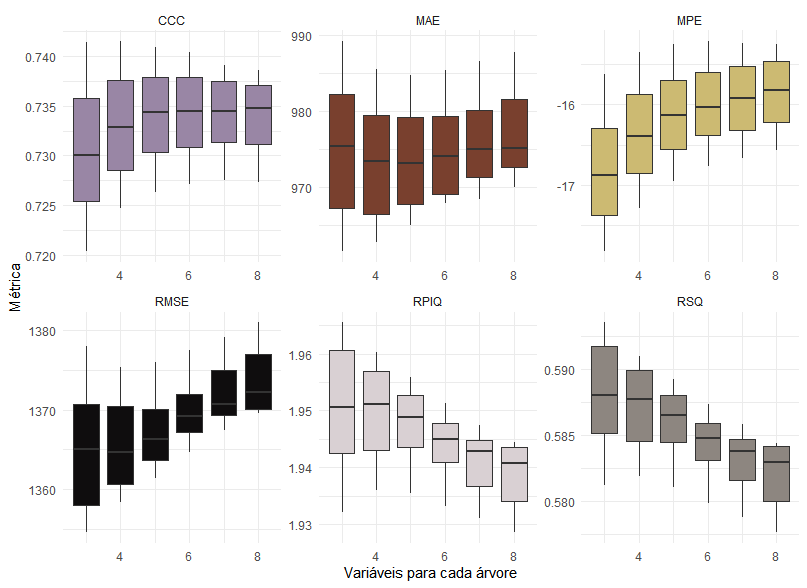
\includegraphics[scale = .72]{imagens/cross_v_mtry.png}}
    \fonte{Elaboração própria.}
\end{figure}

A varredura pelo hiperparâmetro do número de variáveis sugere que ele não é muito determinante para performance. Não há movimentos claros entre as métricas de melhora ou piora, como mostramos na Figura 13. Poucas variáveis por árvore incluem tanto os melhores quanto os piores modelos, como mostramos na Tabela 4. Isso sugere que a amostra mínima para gerar folha é um hiperparâmetro mais relevante. De fato é:


\begin{figure}[H]
    \centering
    \captionbox{Resumo de métricas de performance variando a amostra mínima para criar uma folha.  }{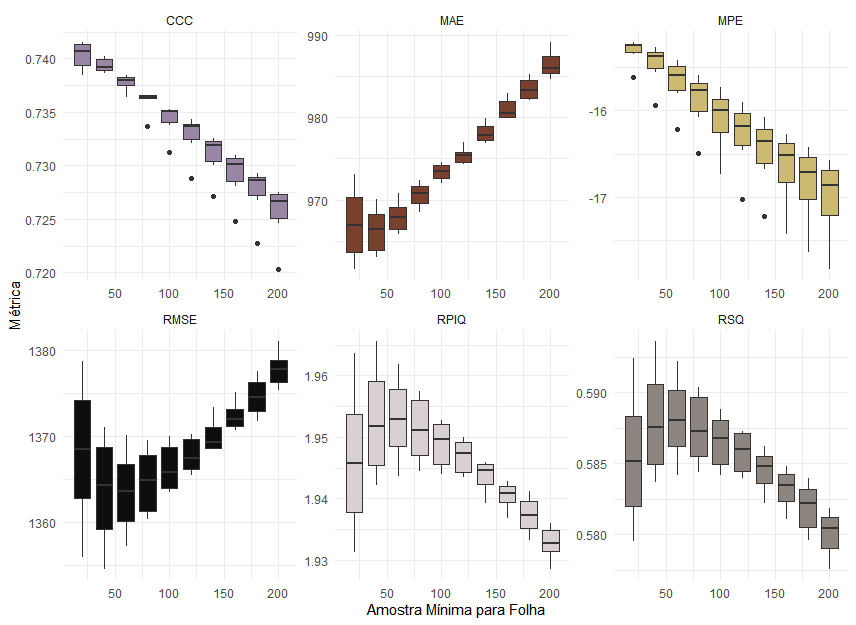
\includegraphics[scale = .70]{imagens/crossv_min.png}}
    \fonte{Elaboração própria.}
\end{figure}

\begin{table}[H]

\caption{\label{tab:tabela_metricas}Melhor modelo de acordo com cada métrica. Elaboração Própria.}
\centering
\begin{tabular}[t]{c|c|c}
\hline
Variáveis por Árvore & Amostra Mínima para Folha & metrica\\
\hline
3 & 20 & RPIQ\\
\hline
4 & 20 & CCC\\
\hline
3 & 20 & MAE\\
\hline
3 & 200 & MPE\\
\hline
3 & 20 & RSQ\\
\hline
3 & 20 & RMSE\\
\hline
\end{tabular}
\end{table}




\section{Computação de Efeitos Marginais}

Primeiro, vamos definir uma referência. Nosso apartamento imaginário tem 92 $m^2$, 3 quartos, 2 banheiros, uma vaga na garagem, fica no oitavo andar, não é mobiliado, fica no Rio de Janeiro e o dono aceita animais. O que seria dele se fosse maior, ou em um andar mais alto?

Ao aplicar o procedimento com um modelo linear, o que temos? Justamente o que modelos lineares deveriam devolver na ausência de termos com interações e funções não-lineares dos regressores originais, efeitos marginais constantes, mostrado na Figura 15.

\begin{figure}[H]
    \label{ols_marg}
    \centering
    
    \captionbox{A aplicação do procedimento em modelos lineares ilustra a primeira hipótese dos modelos.}{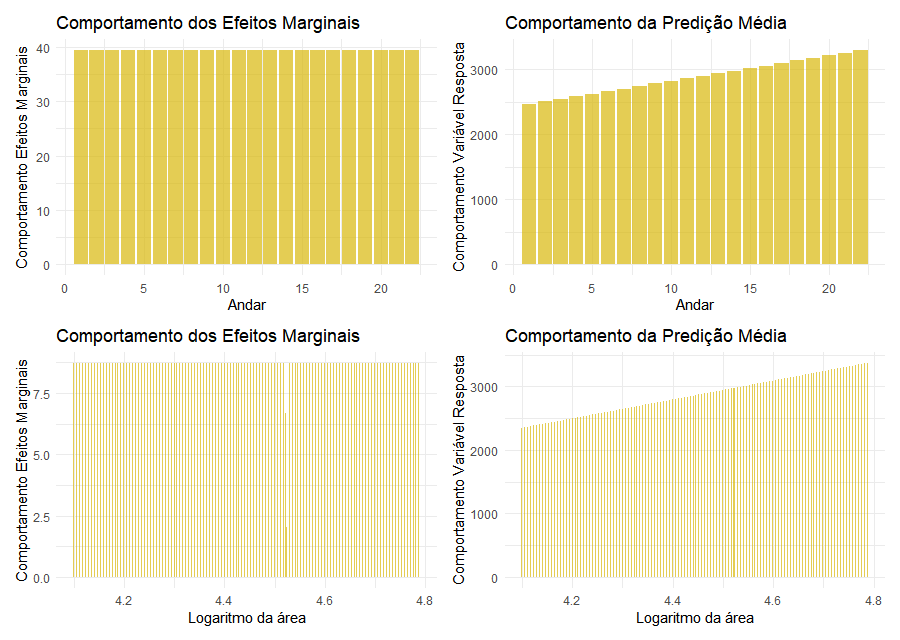
\includegraphics[scale = .68]{imagens/efeitos_marginais_lm.png}}
    \fonte{Elaboração própria.}
\end{figure}

Já em modelos de floresta aleatória a não-linearidade do fenômeno fica evidente. Sair do térreo para o primeiro andar \textit{barateia} um apartamento, presumivelmente porque o benefício de uma vista é quase inexistente embora o custo de subir escada/elevador apareça. Sair do décimo segundo para o décimo terceiro tem um efeito nulo e por vezes negativo. Possivelmente por conta da superstição com o número.

Esse tipo de efeito poderia ser aproximado com regressões pseudo-quantílicas, em que estimamos por OLS um modelo por quantil da amostra ao invés de seguir o procedimento de minimização de valor absoluto da regressão quantílica 'verdadeira'. Uma limitação dessa abordagem é que envolve fatiar a amostra. Mais quantis implicam em amostras sucessivamente menores. Essa limitação não está presente em florestas aleatórias. 

\begin{figure}[H]
    \centering
    \captionbox{Cada curva contém a previsão de uma floresta aleatória distinta.  }{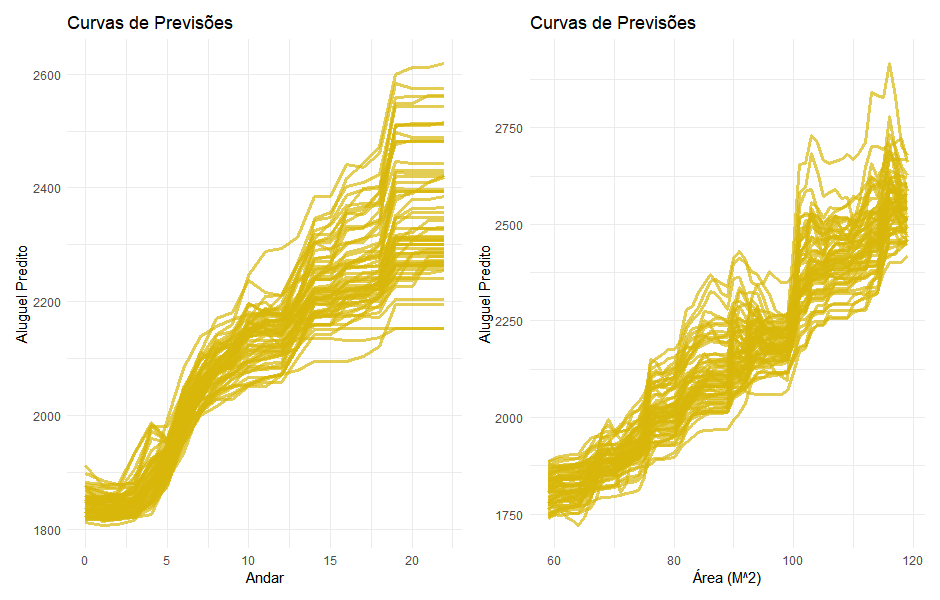
\includegraphics[scale = .60]{imagens/curvas_previsoes_rf.png}}
    \fonte{Elaboração própria.}
\end{figure}



\begin{figure}[H]
    \centering
    
    \captionbox{Em florestas aleatórias a heterogeneidade dos efeitos de tratamento fica evidente.  }{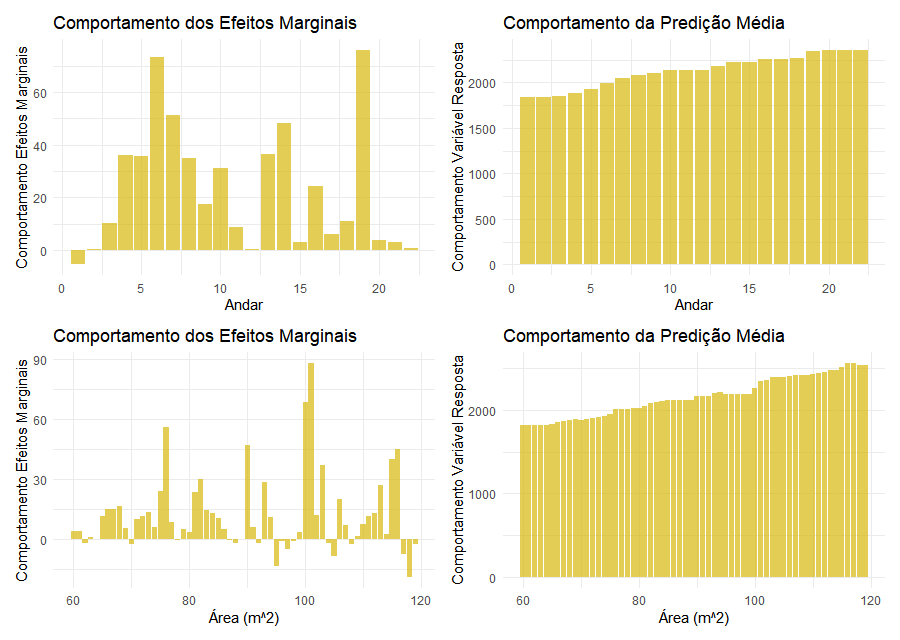
\includegraphics[scale = .60]{imagens/efeitos_marginais_RF.png}}
    \fonte{Elaboração própria.}
\end{figure}



Outra diferença é que modelos lineares são \textit{globais}. Os efeitos marginais independem dos níveis de outros regressores então o salto do térreo para o primeiro andar seria tido como igual para todo apartamento, em toda cidade, de qualquer tamanho. Esse tipo de nuance não é perdida em modelos de florestas aleatórias. 

Embora o exemplo seja em um contexto de regressão, o procedimento não se perde em classificação. A classe predita por uma floresta é a apenas a que recebeu mais votos das árvores individuais. Podemos ler a fração dos votos que a classe mais votada levou como uma probabilidade predita e calcular os efeitos marginais da mesma maneira que faríamos em um caso de regressão, avaliando o efeito sobre a probabilidade predita. Essa mudança para que a saída do modelo seja em probabilidade é trivial na maioria das implementações computacionais destes métodos e não leva a um aumento de complexidade da tarefa.










